\section{Durchführung}
\label{sec:Durchführung}

%Die Funktion eines phasenempfindlichen Gleichrichters für fünf verschiedene Phasen wird verifiziert. 
% Als erstes werden sich die Signale des Funktionsgenerators angeschaut. Dabei werden die beiden Ausgänge verglichen 
% und ihre Eigenschaften überprüft. (unwichtig)

\subsection{Ohne Noise Generator}
\label{sec:eins}
Mit der Schaltung in Abb. \ref{lockin2} soll die Funktionsweise eines Lock-In-Verstärkers getestet werden.
Es wird ein sinusförmiges Signal $U_{Sig}$ von $\SI{1}{\kilo\hertz}$ und 
$\SI{10}{\milli\volt}$ auf den Verstärker gegeben.
Der Ausgang wird mit einem Referenzsignal, welches ein Sinussignal gleicher Frequenz ist, gemischt.
Es werden Aufnahmen der Ausgangssignale für fünf verschiedene eingestellte Phasen gemacht.
\newline
Im nächsten Schritt wird ein Tiefpass, der das Ausgangssignal integriert, 
in den Schaltkreis eingebaut. %"eingebaut"?
% Das neue Ausgangssignal soll überprüft werden. 
Die Ausgangsspannungen werden für verschiedene Phasenverschiebungen gemessen.
Es werden $\num{13}$ Messwerte aufgenommen. 
\begin{figure}
    \centering
    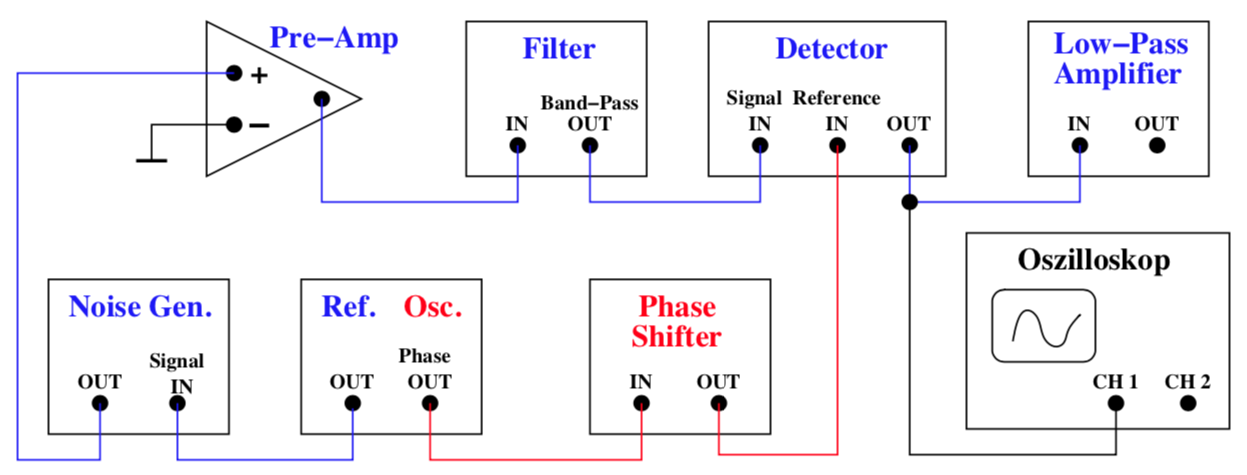
\includegraphics[width=12cm, height=5cm]{build/lockin2.png}
    \caption{Aufbau eines Lock-In-Verstärkers mit Noise Generator.
    Für den Versuchsteil \ref{sec:eins} wird der Noise Generator nicht in die 
    Schaltung eingebaut. In Teil \ref{sec:zwei} wird der Noise Generator in die 
    Schaltung integriert. \cite{V303}}
    \label{lockin2}
\end{figure}

\subsection{Mit Noise Generator}
\label{sec:zwei}
Der Noise Generator wird in die Schaltung integriert (Abb. \ref{lockin2}).
Dieselben Messungen wie zuvor werden noch einmal mit einem Rauschsignal von der Größenordnung der Signalspannung 
durchgeführt.

\subsection{Rauschunterdrückung mit Photodetektorschaltung} %
Im letzten Schritt wird eine Photodetektorschaltung wie in Abb. \ref{lockin3} gebaut.
Die Leuchtdiode wird mit einer Rechteckspannung gespeist und mit einer Frequenz von \SI{100}{\hertz} zum Blinken gebracht.
Mit einer Photodiode wird das ausgesendete Licht anschließend gemessen.
Dabei wird die Lichtintensität als Funktion des Abstands $r$ zwischen LED und Photodiode gemessen.
\begin{figure}
    \centering
    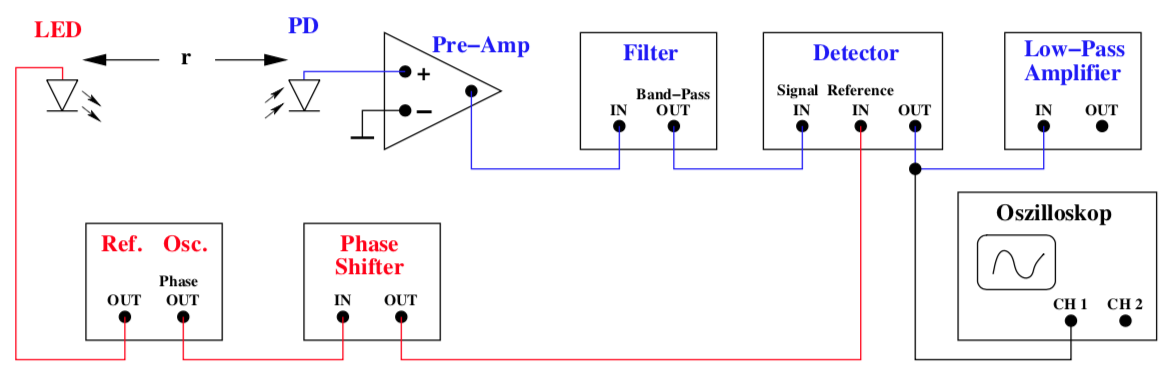
\includegraphics[width=12cm, height=5cm]{build/lockin3.png}
    \caption{Aufbau einer Photodetektorschaltung zur Überprüfung der
    Rauschunterdrückung des Lock-In-Verstärkers. \cite{V303}}
    \label{lockin3}
\end{figure}
